% !TEX encoding = UTF-8 Unicode
\documentclass[a4paper]{article}
\usepackage{geometry}
 \geometry{
 a4paper,
 total={150mm,240mm},
 left=30mm,
 top=30mm,
 }

\usepackage{color}
\usepackage{url}
\usepackage[T2A]{fontenc} % enable Cyrillic fonts
\usepackage[utf8]{inputenc} % make weird characters work
\usepackage{graphicx}
\usepackage[]{algorithm2e}

\usepackage[english,serbian]{babel}
%\usepackage[english,serbianc]{babel} %ukljuciti babel sa ovim opcijama, umesto gornjim, ukoliko se koristi cirilica

\usepackage[unicode]{hyperref}
\hypersetup{colorlinks,citecolor=green,filecolor=green,linkcolor=blue,urlcolor=blue}

\usepackage{listings}

%\newtheorem{primer}{Пример}[section] %ćirilični primer
\newtheorem{primer}{Primer}[section]

\definecolor{mygreen}{rgb}{0,0.6,0}
\definecolor{mygray}{rgb}{0.5,0.5,0.5}
\definecolor{mymauve}{rgb}{0.58,0,0.82}

\lstset{ 
  backgroundcolor=\color{white},   % choose the background color; you must add \usepackage{color} or \usepackage{xcolor}; should come as last argument
  basicstyle=\scriptsize\ttfamily,        % the size of the fonts that are used for the code
  breakatwhitespace=false,         % sets if automatic breaks should only happen at whitespace
  breaklines=true,                 % sets automatic line breaking
  captionpos=b,                    % sets the caption-position to bottom
  commentstyle=\color{mygreen},    % comment style
  deletekeywords={...},            % if you want to delete keywords from the given language
  escapeinside={\%*}{*)},          % if you want to add LaTeX within your code
  extendedchars=true,              % lets you use non-ASCII characters; for 8-bits encodings only, does not work with UTF-8
  firstnumber=1000,                % start line enumeration with line 1000
  frame=single,	                   % adds a frame around the code
  keepspaces=true,                 % keeps spaces in text, useful for keeping indentation of code (possibly needs columns=flexible)
  keywordstyle=\color{blue},       % keyword style
  language=Python,                 % the language of the code
  morekeywords={*,...},            % if you want to add more keywords to the set
  numbers=left,                    % where to put the line-numbers; possible values are (none, left, right)
  numbersep=5pt,                   % how far the line-numbers are from the code
  numberstyle=\tiny\color{mygray}, % the style that is used for the line-numbers
  rulecolor=\color{black},         % if not set, the frame-color may be changed on line-breaks within not-black text (e.g. comments (green here))
  showspaces=false,                % show spaces everywhere adding particular underscores; it overrides 'showstringspaces'
  showstringspaces=false,          % underline spaces within strings only
  showtabs=false,                  % show tabs within strings adding particular underscores
  stepnumber=2,                    % the step between two line-numbers. If it's 1, each line will be numbered
  stringstyle=\color{mymauve},     % string literal style
  tabsize=2,	                   % sets default tabsize to 2 spaces
  title=\lstname                   % show the filename of files included with \lstinputlisting; also try caption instead of title
}

\begin{document}

\title{Podešavanje težina neuronske mreže upotrebom optimizacionog algoritma\\ \small{Seminarski rad u okviru kursa\\Računarska inteligencija\\ Matematički fakultet}}

\author{Nikola Stamenić, Lea Petković\\ mi16177@alas.matf.bg.ac.rs, mi16163@alas.matf.bg.ac.rs}

%\date{9.~april 2015.}

\maketitle

\abstract{
U ovom tekstu je ukratko prikazana osnovna forma seminarskog rada. 

\tableofcontents

\newpage

\section{Uvod}
\label{sec:uvod}

Ovde ide neki uvod

\section{Neuronske mreže}
\label{neuronskemreze}

Neuronska mreža (eng. \emph{Artificial Neural Networks, ANN}) je sistem koji vrši mapiranje između ulaza i izlaza problema.
Neuronske mreže zapravo predstavljaju parametrizovanu reprezentaciju koja se može koristiti za aproksimaciju raznih funkcija \cite{hindawi}.
Matematičkom optimizacijom nekog od kriterijuma kvaliteta vrši se pronalaženje odgovarajućih parametara. 

Neuronske mreže uče informacije kroz proces treniranja u nekoliko iteracija. Kada je proces učenja završen, 
neuronska mreža je spremna i sposobna da klasifikuje nove informacije, predvidi ponašanje, ili aproksimira nelinearnu funkciju problema. 
Njena struktura sastoji se od skupa neurona, predstavljenih
funkcijama, koji su međusobno povezani sa ostalim neuronim organizovanim u slojevima. 

Struktura neuronske mreže se razlikuje po broju slojeva. Prvi sloj jeste ulazni sloj, poslednji sloj jeste izlazni, a svi slojevi između se nazivaju skrivenim
slojevima. Slojevi su međusobno potpuno povezani. Slojevi komuniciraju zahvaljujući tome što je izlaz svakog neurona, iz prethodnog sloja, povezan sa
ulazima svih neurona iz narednog sloja. Jačina veza kojom su neuroni međusobno povezani se naziva težinski faktor (eng. \emph{weight}). Najčešće ima
3 sloja.

Postoje različite vrste neuronskih mreža. Mozemo ih klasifikovati prema: broju slojeva (jednoslojne i višeslojne), vrsti veza između neurona, smeru
prostiranja informacija (neuronske mreže sa propagacijom unapred ili unazad) \cite{website}, vrsti podataka itd. 

Njihove primene su mnogobrojne, obzirom da predstavljaju najčešće primenjivanu metodu mašinskog učenja. Neke od primena su: kategorizacija teksta,
medicinska dijagnostika, prepoznavanje objekata na slikama, autonomna vožnja, igranje igara poput igara na tabli ili video igara, mašinsko prevođenje
prirodnih jezika, prepoznavanje rukom pisanih tekstova itd. 

\subsection{Keras Pajton biblioteka}
\label{subsec:keras}

Keras je biblioteka za neuronske mreže, napisana u Pajtonu. Keras radi na platformi za mašinsko učenje  \textit{TensorFlow}.
Razvijena je sa ciljem da omogući brzo eksperimentisanje sa neuronskim mrežama \cite{keraswebsite},
da bude razumljiva, modularna i proširiva.

Pored, već pomenute, \textit{TensorFlow} platforme, ova biblioteka radi i na: \textit{Microsoft Cognitive Toolkit, R, Theano, ili PlaidML} platformama. 
Nastala je kao deo istraživanja u okviru projekta ONEIROS (eng. \emph{Open-ended Neuro-Electronic Intelligent Robot Operating System}), 
a njen autor i održavaoc je gugl inženjer -  François Chollet.
% \begin{verbatim}
% ščćžđ
% \end{verbatim}

\section{Optimizacija rojem čestica}
\label{subsec:pso}
U ovoj sekcije biće objašnjen sam algoritam optimizacije rojem čestica. Najviše vremena biće posvećeno originalnom algoritmu PSO,
a kao i drugoj generaciji algoritma PSO (eng. \textit{The Secong Generation of PSO}), kao i novom modelu algoritma PSO 
(eng. \textit{A New Model of PSO}).


\subsection{Originalni algoritam PSO}
\label{subsec:opso}
Algoritam PSO (eng. \textit{Particle Swarm Optimization}) je metod za optimizaciju neprekidne nelinearne funkcije, koji je predložio Eberhart.
Sam algoritam je inspirisan posmatranjem socijalnog i kolektivnog ponašanja u kretanju jata ptica pri potrazi za hranom ili preživaljavanjem.
PSO je nadahnut kretanjem najboljeg člana populacije i njegovog iskustva. Metafora govori da se skup rešenja kreće prostorom pretrage sa ciljem da nađe što bolju poziciju, rešenje \cite{hindawi}.
\\
Populacijom se smatra grupa čestica \textit{i} gde svaka predstavlja poziciju \textbf{\textbf{$x_i \in R^D$, i = 1,...,M}} u višedimenzionom prostoru.
Čestice se evaluiraju u posebnoj funkciji optimizacije, kako bi se odredila njihova prilagođenost i sačuvala najbolja vrednost. Svaka čestica se kreće po
prostoru pretrage u zavisnosti od funkcije brzine \textbf{$v_i$} koja u obzir uzima globalno najbolju poziciju u populaciji ($p_g \in R^D$ - socijalna
komponenta) kao i najbolju poziciju date čestice ($p_g \in R^D$ - kognitivna komponenta). Čestice će se kretati u svakoj iteraciji na drugu poziciju,
dok ne dostignu optimalnu poziciju. U svakom momentu \textit{t}, brzina čestice \textit{i} se ažurira koristeći: 
\begin{center}
\textbf\textit{$v_i(t+1) = \omega v_i(t) + c_1 r_1(p_i (t) - x_i (t)) + c_2 r_2 (p_g (t) - x_i (t))$}
\end{center}
gde je $\omega$ inertna težina i obično je postavljena da varira linearno od 1 do 0 tokom iteracije, $c_1$ i $c_2$ su koeficijenti ubrzanja, $r_1$ i $r_2$
su slučajni brojevi iz uniformne (0,1) raspodele. Ubrzanje \textbf{$v_i$} je ograničeno između [$v_min, v_max$]. Ažuriranjem ubrzanja na ovaj 
način dozvoljavamo jedinki $i$ da traži najbolju poziciju \textbf{$p_i(t)$}, dok se najbolje globalno rešenje računa:\cite{hindawi}
\begin{center}
\textbf\textit{$x_i(t+1) = x_i(t) + v_i(t+1)$}
\end{center} 
% Optimizacija rojem čestica se može prikazati sledećim pseudokodom:

%Za sva rešenja (čestice)  𝑖  iz skupa rešenja (roja)  𝑋 :

%Izabrati koordinate vektora  𝑥𝑖  uniformno iz intervala  (𝑙,𝑢) 
%𝑝𝑖=𝑥𝑖 
%Ako je  𝑓(𝑥𝑖)<𝑓(𝑔)  tada  𝑔=𝑥𝑖 
%Označiti koordinate vektora  𝑣𝑖  da su jednaki nuli ili uniformno iz %intervala  (−|𝑢−𝑙|,|𝑢−𝑙|) 
%Dok nije ispunjen kriterijum zaustavljanja:

%Za sve čestice  𝑖  iz roja  𝑋 :
%Izabrati brojeve  𝑟𝑔  i  𝑟𝑝  uniformno iz intervala  (0,1) 
%𝑣𝑖=𝑐𝑣𝑣𝑖+𝑐𝑝𝑟𝑝(𝑝𝑖−𝑥𝑖)+𝑐𝑔𝑟𝑔(𝑔−𝑥𝑖) 
%𝑥𝑖=𝑥𝑖+𝑣𝑖 
%Ako je  𝑓(𝑥𝑖)<𝑓(𝑝𝑖)  tada  𝑝𝑖=𝑥𝑖 
%Ako je  𝑓(𝑥𝑖)<𝑓(𝑔)  tada  𝑔=𝑥𝑖 
%Rešenje je vektor  𝑔 , a vrednost rešenja broj  𝑓(𝑔)


\subsection{Druga generacija PSO algoritma}
\label{subsec:sgpso}
Druga generacija PSO algoritma je unapređenje originalnog PSO algoritma, koja u obzir uzima tri aspekta: lokalni optimum svih jedinki,
globalno najbolje rešenje, i novi koncept - geometrijski centar optimalne populacije. Autor knjige \textit{"{}Second Generation Particle Swarm Optimization"} objašnjava da ptice održavaju 
određenu distancu između centra jata (hrane). Jata ptica uvek ostaju u istom regionu neko vreme, tokom kojeg će centar jata ostati
nepomeren u očima jedinki. Nakon toga, jato se kreće na sledeći region, tada sve jedinke moraju održati određenu distancu sa centrom jata.

\subsection{Novi model PSO-a}
\label{subsec:nmpso}
Ovaj algoritam je predložen od strane Garoa (eng. \textit{Garro}), a on ga je bazirao na osnovu ideja drugih autora koji su predlagali unapređenje
originalnog PSO algoritma. 
Shi i Eberhart su predlagali linearno variranje inertnih težina kroz generacije, što je znatno unapredilo performanse originalnog PSO algoritma.
Yu je razvio strategiju da kada se kroz generacije globalno najbolje rešenje ne poboljšava, svaka jedinka \textit{$i$} biva izabrana sa predefinisanom
verovatnoćom a zatim dodat slučajni šum svakom vektoru brzine dimenzije $v_i$ izabrane jedinke \textit{$i$}.
Bazirano na nekim evolutivnim shemama Genetičkih Algoritama, nekoliko efektnih mutacija i ukrštanja su predložene za PSO.

\section{Podešavanje težina neuronske mreže pomoću optimizacije rojem čestica}
\label{sec:podesavanjetezina}

Treniranje neuronske mreže, odnosno podešavanje težina, izvršeno je pomoću optimizacije rojem čestica. 
Napravljena je troslojna neuronska mreža (ulazni, skriveni i izlazni sloj) pomoću Keras biblioteke u Pajtonu, 
pomoću koje se rešavaju klasifikacioni problemi. Dve trećine podataka korišćene su za trening podatke, a ostatak čini test podatke. 
Skriveni sloj sadrži 100 jedinica/čvorova, dok je broj izlaza ekvivalentan b
roju različitih klasa u odgovarajućem skupu podataka. Kao metrika korišćena je preciznost (eng. \emph{accurancy}). 

Kao što je ranije napomenuto, ANN trenirana je pomoću PSO algoritma. PSO koristi 30 čestica, prolazi kroz 300 iteracija i šalju se trening 
podaci i neuronska mreža. Težine neuronske mreže predstavljaju pozicije čestica. Inicijalne težine biraju se nasumično unutar intervala [-2, 2], 
a ažuriranje težina se vrši prema formuli: 
\begin{center}
{$x_i(t+1) = x_i(t) + v_i(t+1)$}
\end{center}
objašnjenoj u poglavlju \ref{subsec:opso}. Parametri c1, c2 i w izabrani su u odnosu na vrednosti istih tih parametara u radu \cite{hindawi},
odnosno w je 0.3, dok su c1 i c2 za 0.5 manji, jer tako algoritam daje bolje rezultate. 

Kao funkcija cilja korišćena je preciznost. Takođe, u cilju izbegavanja zaglavljivanja u lokalnom minimumu algoritam se pokreće nekoliko puta i 
pozicije najgorih 5 čestica se nasumično menjaju. Najbolja čestica je upravo ona sa najvećom preciznošću.

\subsection{Rezultati}
\label{rezultati}

U ovoj sekciji biće predstavljeni eksperimentalni rezultati dobijeni nad skupovima: Iris, Breast Cancer i Wine, kao i 
upoređeni sa rezultatima drugih istraživača koji su se bavili ovom temom i koristili navedene skupove \cite{hindawi}. 
U nastavku sledi više o rezultatima na svakom od njih pojedinačno.

\subsubsection{Skup Iris}
\label{iris}

Ovaj skup podataka nalazi se u Pajton paketu za mašinsko učenje: Scikit-learn. Sastoji se od 3 vrste cveta Iris - Setosa, Versicolour, Virginica. 
Sadrži 150 instanci i ima 5 atributa koji predstavljaju dužinu i širinu latica (eng. \emph{petal length, petal width}), dužinu čašičnog listića 
(eng. \emph{sepal length, sepal width}) i vrstu kojoj cvet pripada (eng. \emph{species}). 


\subsubsection{Skup Breast cancer}
\label{breast}

\subsubsection{Skup Wine}
\label{wine}


\begin{figure}[h!]
\begin{center}
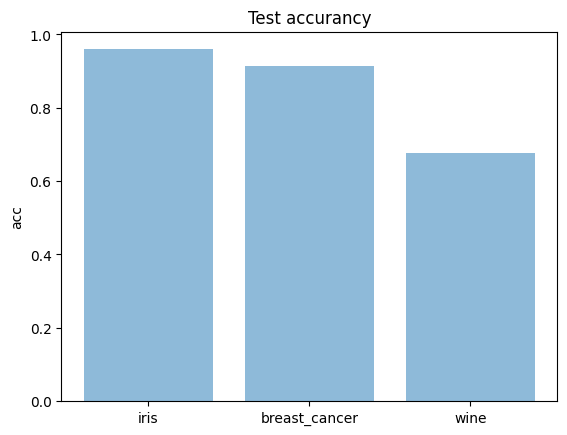
\includegraphics[scale=0.5]{download.png}
\end{center}
\caption{Preciznost na test podacima skupova: iris, breast cancer i wine.}
\label{fig:preciznost}
\end{figure}

\textit{Ovo poglavlje sadrži tabele i grafike kojim upoređujete vaš pristup sa drugim pristupima iz literature. Pronaći relevantne test 
primere (instance) I testirati predloženu metodu (metode) na njima, ukoliko su dostupne. Ako ne možete da dođete do test primera iz 
literature, kreirajte na osnovu opisa iz radova test primere koji su im slični. Testirajte vaše metode pod sličnim uslovima kao i autori iz 
literature. Pri demonstraciji rada metode uvek pokazati kako vaša metoda radi na na jednostavnim test primerima koji se mogu 
vizualizovati. Specijalno, ako ne upoređujete rešenje sa drugim rešenjima, možete komentarisati efikasnost algoritma i procenijvati
kvalitet tako što ga upoređujete sa drugim pristupima koje ste sami razvili (npr. algoritmom potpune pretrage, eng. brute-force u slučaju
da radite optimizacionu tehniku). Budite objektivni i pošteni u prikazu svojih rezultata i jasno naznačite ako vaš pristup nije bolji 
(što je vrlo verovatno) od onih koji su predloženi u literaturi. U okviru ovog poglavlja opišite i eksperimentalno okruženje u kojem 
ste testirali vaš program, karakteristike hardvera, operativni sistem, kompajler, itd. }



\section{Zaključak}
\label{sec:zakljucak}

Ovde pišem zaključak. 


\addcontentsline{toc}{section}{Literatura}
\appendix
\bibliography{seminarski} 
\bibliographystyle{plain}

\appendix
\section{Dodatak}
Ovde pišem dodatne stvari, ukoliko za time ima potrebe.


\end{document}
